\begin{figure}[t]
  \begin{center}
    \begin{tabular}{c}
      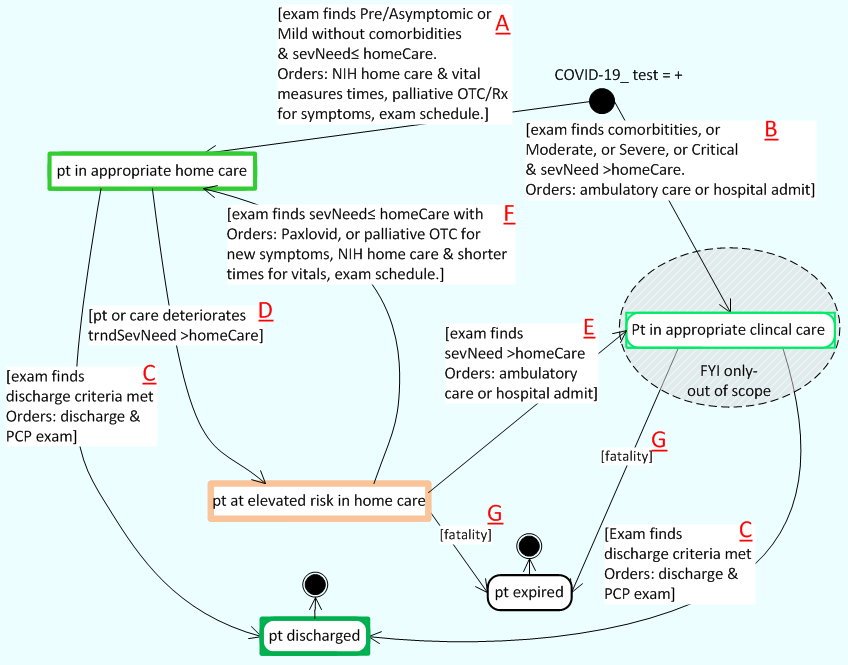
\includegraphics[scale=0.4]{cwp.png}
    \end{tabular}
  \end{center}
\caption{The \href{https://github.com/ericmercer/SPIN-bpmn-cwp-verification-paper/blob/main/26-Oct-2021-CWP.png}{CWP} for remote COVID-19 patient care.}
\label{fig:cwp}
\end{figure}

A fundamental aspect of RPM is the establishment and maintenance of providers' awareness of their patient’s condition and risk during home care.
Medical use and testing of \phware for this purpose will require design of an end-to-end system that must implement appropriate policy for risk awareness for COVID-19 patients during home care, and for transitions to-and-from their different levels of care.
We call this CWP \emph{actionable risk awareness} and the policy is adapted from \emph{NIH COVID-19 Treatment Guidelines} published by the U.S. National Institute of Health \cite{NIH}.
The \emph{Guidelines} detail five levels of COVID-19 severity and appropriate treatments for each level.
In order to apply them as technology-independent CWP they are summarized and represented here as the finite state machine in \figref{fig:cwp}.

The finite state machine is composed of the relevant states patients can occupy, their associated risks, and the transition conditions among them. They give precise, rigorous meaning to the abstract concept of \emph{actionable risk awareness} as a set of transformations on a complex object of work that is shared by the activities in a distributed cognitive system.

In the initial state of \figref{fig:cwp} all patients have tested positive for COVID-19. The arc labeled letter-\textbf{B} occurs when an exam finds patients have severity needs that are greater than home care (\emph{sevNeed $>$homeCare}) and are ordered to ambulatory care or hospital admission.
The remaining focus of Fig.1 is on patients who qualify for home care, with exam findings that are presymptomatic, asymptomic, or have only mild symptoms and no comorbidities (letter-\textbf{A}).
They are ordered to home care and vitals RPM because the treatment that can be carried out there is equal-to-or-greater than their severity level needs (\emph{$sevNeed \le homeCare$}).
Vital signs are measured at instructed times for analysis and RPM, thereby establishing an important aspect of \emph{actionable risk awareness}.
Patients remain in home care until they either meet discharge criteria (letter-\textbf{C}); or the trend of their condition or home care deteriorates  (\emph{trndSevNeed $>$homeCare}) putting them at elevated risk (letter-\textbf{D}).

Patients must not remain in care that cannot meet their needs because there is a direct path from that state to fatality (letter-\textbf{G}).
From \textbf{D} a near-future exam must determine if they are ordered to clinical care (letter-\textbf{E}) or whether they can be restored to \emph{$sevNeeds\le homeCare$} with increased RPM or medication for new symptoms (letter-\textbf{F}).
From ambulatory or hospital care patients can be discharged at \textbf{C}, or expire at \textbf{G}.

The validation of the CWP for \phware merits explanation.
The \emph{NIH Guidelines} are an authoritative source, but the finite state diagram only summarizes key sections relevant to states and transitions. 
The graphical representation serves as sort of story board that allowed it to be critiqued by doctors. 
One example critique led us to add more content to letter-A about the types of home care.  
For another, we added the primary care provider's exam (PCP exam) as part of discharge orders. The revised version might be adjusted for some clinics to meet local resource limits, but now serves as a core requirement. 

The requirement specified by the CWP is the medical care problem that must be solved by a system design for vital signs RPM.
Importantly, the specification is independent of any technology beyond vital signs, and could be met with a variety of systems designed around other technologies.  
As presented next, this same technical independence also allows the CWP to be translated into LTL, then serve as the criterial property for model-checking to verify the integrated design.
